

\documentclass[18pt]{beamer}

\usepackage[utf8]{inputenc}
\usepackage{graphicx}
\graphicspath{ {images/} }

\usepackage{templates/beamerthemekit}
%\usepackage{templates/beamerthemekitwide}

%% TITLE PICTURE

% if a custom picture is to be used on the title page, copy it into the 'logos'
% directory, in the line below, replace 'mypicture' with the 
% filename (without extension) and uncomment the following line
% (picture proportions: 63 : 20 for standard, 169 : 40 for wide
% *.eps format if you use latex+dvips+ps2pdf, 
% *.jpg/*.png/*.pdf if you use pdflatex)

%\titleimage{Folientitelbild_wide}

%% TITLE LOGO

% for a custom logo on the front page, copy your file into the 'logos'
% directory, insert the filename in the line below and uncomment it

%\titlelogo{infofak}

% (*.eps format if you use latex+dvips+ps2pdf,
% *.jpg/*.png/*.pdf if you use pdflatex)

\usepackage{multicol}
\usepackage{xcolor}
\usepackage[ruled,linesnumbered,vlined,boxed,commentsnumbered]{algorithm2e}
\usepackage{soul}
\usepackage{multirow}
\definecolor{kit}{RGB}{21,135,118}

% the presentation starts here

\title[Flexible User-Friendly Trip Planning
Queries]{Bachelor's Thesis \\ Flexible User-Friendly Trip Planning Queries}
\subtitle{Adviser: Saeed Taghizadeh}
\author{Violina Zhekova}

\institute{Institute for Program Structures and Data Organization (IPD), Chair Prof. B{\"o}hm}

\begin{document}

\SetKwFunction{NN}{NN}
\SetKwFunction{KNN}{kNN}
\SetKwBlock{A}{a)}{end}
\SetKwBlock{B}{b)}{end}
\SetKwFunction{trim}{trim}
\SetKwFunction{caseBefore}{caseBefore}
\SetKwFunction{caseContaining}{caseContaining}
\SetKwFunction{caseAfterOrContaining}{caseAfterOrContaining}
\SetKwFunction{caseAfter}{caseAfter}

% change the following line to "ngerman" for German style date and logos
\selectlanguage{english}

%title page
\begin{frame}
	\titlepage
\end{frame}

%table of contents
\begin{frame}{Outline}
	\begin{multicols}{2}
		\tableofcontents
	\end{multicols}
\end{frame}


\section{Motivation}
	\begin{frame}{Motivation}
	
		\begin{itemize}
			\item \textit{Sequenced Route Queries} (SRQ) - finding routes passing through multiple \textit{Points of Interest} (PoIs)
			\item Advances in \textit{Location Based Services} (LBS) and \textit{Geographic Information System} (GIS) applications (e.g. logistics and supply chain management)
			\item \underline{Aim}: Designing a language to enable the user to express his query requirements in a flexible manner
		\end{itemize}
		
		\begin{figure}[h]
			
\includegraphics[scale=0.2]{Motivation.jpg}
		\end{figure}
	
	\end{frame}

\section{Related Work}
	\begin{frame}{Related work}
	
		\begin{itemize}
			\item Vector vs. metric spaces
			\item \textit{Trip Planning Queries} (TPQ) \cite{tpq}
			\item The \textit{Optimal Sequenced Route} (OSR) Query \cite{osr}
			\item The Skylyne concept applied to SRQ \cite{skyline}
			\item Considering multiple factors of a route – rating of PoIs, distance and category weights, dynamic factors (e.g. traffic information) \cite{factors}
			\item SRQ issued by users moving along a route \cite{moving}
			\item \textit{Multi-rule Partial Sequenced Route} (MRPSR) Query \cite{multi}
		\end{itemize}
	
	\end{frame}

\section{Example}
	\begin{frame}{Example}
	
		\begin{itemize}
			\item \textbf{Category sequence}: (restaurant, bank, movie theater, restaurant) 
			\textbf{Condition}: equal restaurants
			\pause
			\item \textit{Optimal Sequenced Route} (OSR): $(r_1, b_1, mt_1, r_2)$, length: 11 (shown with \textcolor{red}{red} lines)
			\item Optimal route with equal restaurants: $(r_1, b_1, mt_1, r_1)$, length: 12 (shown with dashed lines)
		\end{itemize}
	
		\only<2>{\begin{figure}[h]
			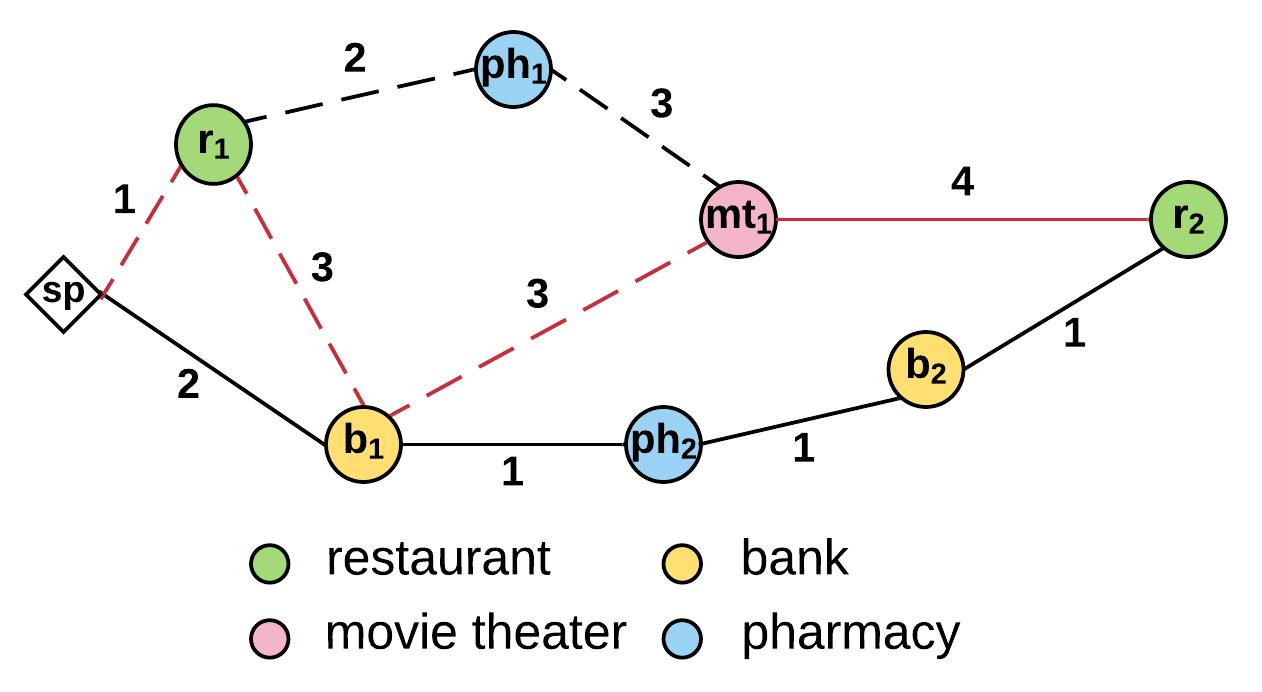
\includegraphics[scale=0.7]{Example_beamer.png}
		\end{figure}}
	
	\end{frame}

\section{Problem Definition}
	\begin{frame}{Problem definition}
	
		\begin{itemize}
			\item \textbf{Problem}: Need for flexibility in route finding queries
			\item \textbf{Solution}: Developing a query language operators to fulfill the essential user's requirements:
			\begin{itemize}
				\item Relationships among the PoIs
				\item Order and priority of the PoIs
				\item Expressing multiple travel variations
				\newline
			\end{itemize}
		    \pause
		    \item Proposing four essential operators: "equality" operator, "inequality" operator, "or" operator, "order" operator
		    \item Making use of existing approaches (PNE (\textit{Progressive Neighbor Exploration}) \cite{osr}) to transform the complex user query 
		\end{itemize}
	
	\end{frame}

\section{Introducing the Operators}

	\subsection{Equality operator}
		\begin{frame}{"Equality" operator}
			
			\begin{itemize}
				\item \textit{Input}: A category sequence $M = (c_1, c_2, ..., c_l)$, a starting point $sp$ in ${\rm I\!R}^2$ and indices of the equal PoIs $i$ and $j$, where $c_i = c_j$
				\item \textit{Output}: Optimal route $R = (r_1, r_2, ..., r_l)$, where $r_i = r_j$ \newline
				\item \textbf{Proposed approach}: uses the Progressive Neighbor Explorator (PNE) as its base to upgrade on and extends it with a heuristic approach to shrink the search space
				\item \textbf{Baseline/trivial approach}: extends the PNE with forcing the PoIs $r_i$ and $r_j$ to be equal; does not use optimization techniques
			\end{itemize}
			
		\end{frame}
	
		\begin{frame}{Heuristic}
			Given a sequence of categories $M = (c_1, c_2, ..., c_l)$ and a PSR $R' = (r_1, r_2, ..., r_k)$ the \textbf{\textit{heuristic}} for this route is defined as: 
			
			\begin{equation}
			h(R') = \max_{i \in [k+1, l]} nearestNeighbor(r_k, C_{M_{i}})
			\end{equation}
			
			\begin{itemize}
				\item Informal: The heuristic of a certain PSR is the maximum distance out of the distances to the nearest PoIs from the set of categories that are yet to be expanded. 
			\end{itemize}
			\pause
			The \textbf{\textit{lower bound}} of a PSR $R'$ represents the sum of its length and its heuristic:
			
			\begin{equation}
			LB(R') = length(R') + h(R')
			\end{equation}
			
			\begin{itemize}
				\item The proposed algorithm uses a heap, sorted by the lower bound of the routes
			\end{itemize}
		\end{frame}
	
		\begin{frame}{Example: Step 1}
	$M = (r, b, mt, r)$, $EQUAL(0, 3)$
	
	\begin{itemize}
		\item Optimal route found with PNE: $(r_1, b_1, mt_1, r_2)$
		\item Dummy SR: $(r_1, b_1, mt_1, r_1)$; Upper Bound $UB = length(dummySR)$
	\end{itemize}

	\begin{figure}[h]
		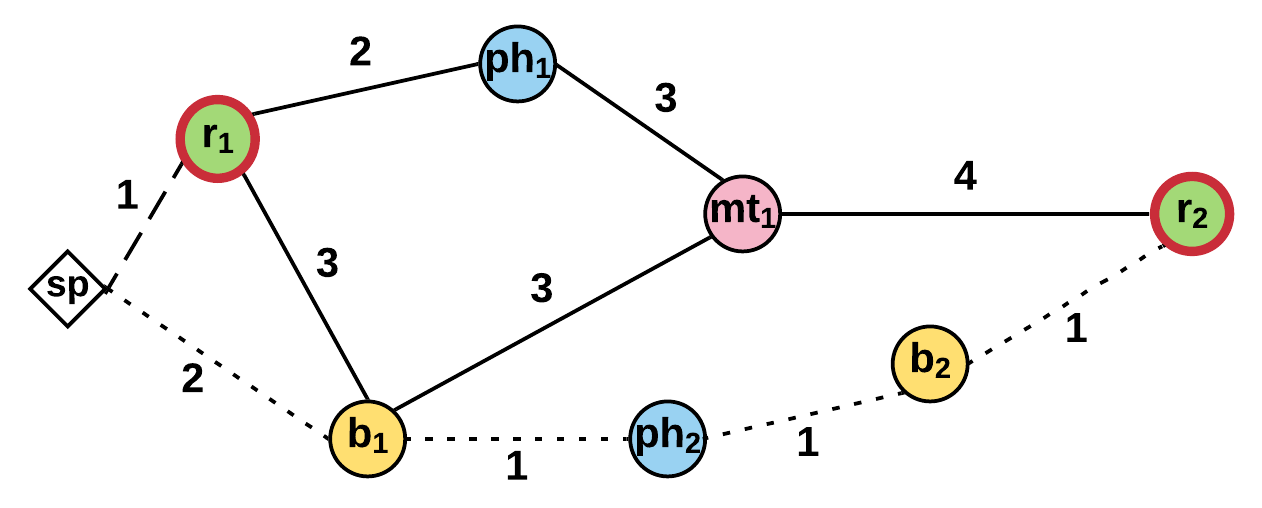
\includegraphics[scale=0.8]{Example_EO_1.png}
	\end{figure}
	
	\begin{table}[h]
		\centering
		\begin{tabular}{ |l|p{10cm}| } 
			\hline
			Step & Heap contents (PSR $R : length(R), heuristic(R)$) \\
			\hline
			\textcolor{red}{1} & \textcolor{red}{$(r_1 : 1, 5)$}, \textcolor{red}{$(r_2 : 5, 4)$} \\ 
			\hline
		\end{tabular}
	\end{table}
		
\end{frame}

\begin{frame}{Example: Step 2}
	$M = (r, b, mt, r)$, $EQUAL(0, 3)$

	\begin{figure}[h]
		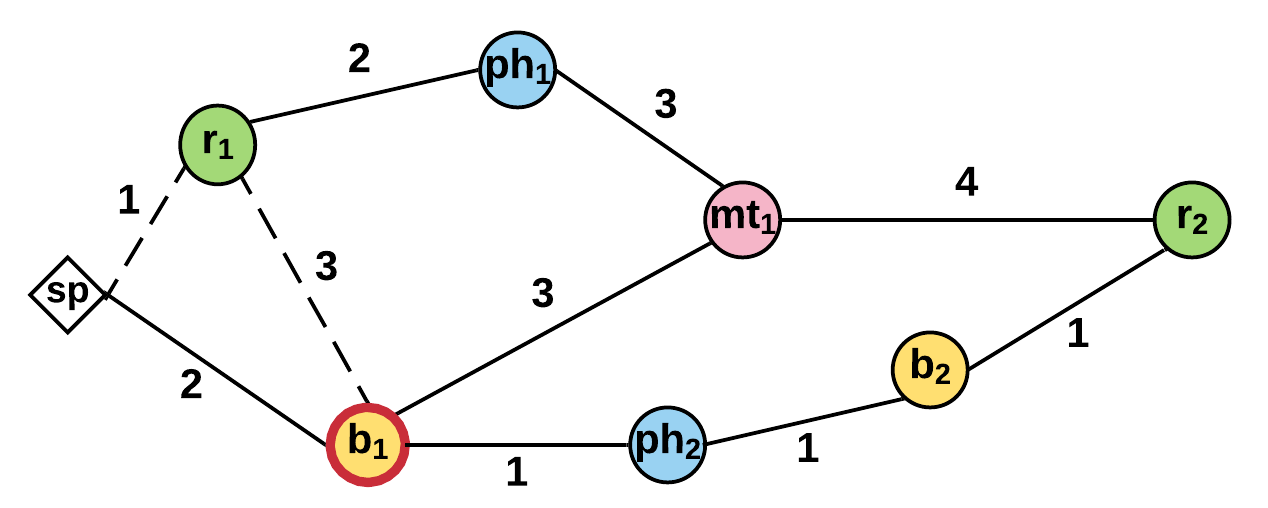
\includegraphics[scale=0.8]{Example_EO_2.png}
	\end{figure}
	
	\begin{table}[h]
		\centering
		\begin{tabular}{ |l|p{10cm}| } 
			\hline
			Step & Heap contents (PSR $R : length(R), heuristic(R)$) \\
			\hline
			1 & $(r_1 : 1, 5), (r_2 : 5, 4)$ \\ 
			\hline
			\textcolor{red}{2} & \textcolor{red}{$(r_1, b_1 : 4, 3)$}, $(r_2 : 5, 4)$ \\ 
			\hline
		\end{tabular}
	\end{table}

\end{frame}

\begin{frame}{Example: Step 8}
	$M = (r, b, mt, r)$, $EQUAL(0, 3)$
	
	\begin{figure}[h]
		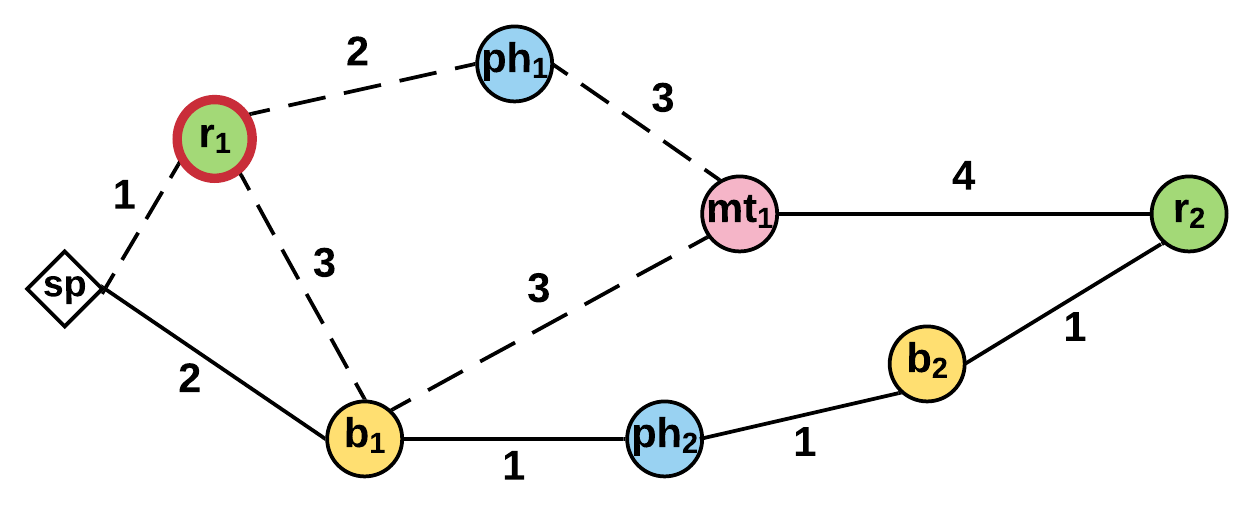
\includegraphics[scale=0.8]{Example_EO_8.png}
	\end{figure}
	
	Candidate SR: \textcolor{red}{$(r_1, b_1, mt_1, r_1 : 12, 0)$}
	
	\begin{table}[h]
		\centering
		\begin{tabular}{ |l|p{10cm}| } 
			\hline
			Step & Heap contents (PSR $R : length(R), heuristic(R)$) \\
			\hline
			7 & $(r_1, b_1, mt_1 : 7, 5), (r_2, b_1, mt_1 : 11, 4), (r_2, b_2, mt_1 : 11, 4),$ \newline $(r_1, b_2, mt_1 : 11, 5)$ \\ 
			\hline
			\textcolor{red}{8} & $(r_2, b_1, mt_1 : 11, 4), (r_2, b_2, mt_1 : 11, 4), (r_1, b_2, mt_1 : 11, 5)$ \\ 
			\hline
		\end{tabular}
	\end{table}

\end{frame}

\begin{frame}{Example: Step 9}
	$M = (r, b, mt, r)$, $EQUAL(0, 3)$
	
	\begin{figure}[h]
		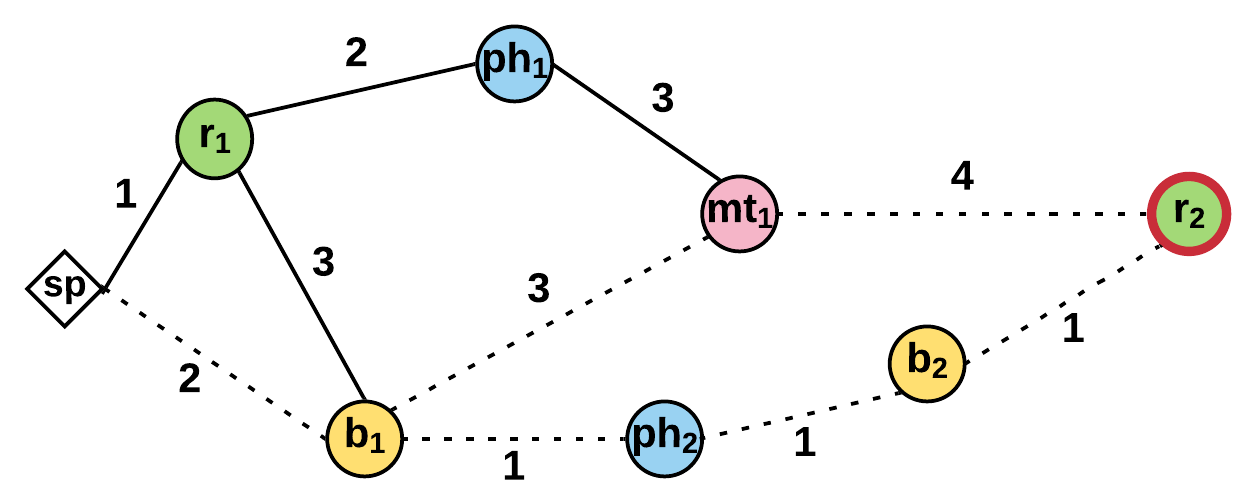
\includegraphics[scale=0.8]{Example_EO_9.png}
	\end{figure}
	
	Candidate SR: \textcolor{red}{$(r_2, b_1, mt_1, r_2 : 15, 0)$}

	\begin{table}[h]
		\centering
		\begin{tabular}{ |l|p{10cm}| } 
			\hline
			Step & Heap contents (PSR $R : length(R), heuristic(R)$) \\
			\hline
			8 & $(r_2, b_1, mt_1 : 11, 4), (r_2, b_2, mt_1 : 11, 4), (r_1, b_2, mt_1 : 11, 5)$ \\ 
			\hline
			\textcolor{red}{9} & $(r_2, b_2, mt_1 : 11, 4), (r_1, b_2, mt_1 : 11, 5)$ \\ 
			\hline
		\end{tabular}
	\end{table}

\end{frame}

%\begin{frame}{Example}
%
%	\begin{table}[]
%		\centering
%		\begin{tabular}{ |l|p{10cm}| } 
%			\hline
%			Step & Heap contents (PSR $R : length(R), heuristic(R)$) \\
%			\hline
%			1 & $(r_1 : 1, 5), (r_2 : 5, 4)$ \\ 
%			\hline
%			2 & $(r_1, b_1 : 4, 3), (r_2 : 5, 4)$ \\ 
%			\hline
%			3 & $(r_2 : 5, 4), (r_1, b_2 : 6, 5), (r_1, b_1, mt_1 : 7, 5)$ \\ 
%			\hline
%			4 & $(r_1, b_2 : 6, 5), (r_2, b_2 : 6, 5), (r_1, b_1, mt_1 : 7, 5) $ \\ 
%			\hline
%			5 & $(r_2, b_2 : 6, 5), (r_1, b_1, mt_1 : 7, 5)$,  \newline $(r_1, b_2, mt_1 : 11, 5)$ \\ 
%			\hline
%			6 & $(r_2, b_1 : 8, 3), (r_1, b_1, mt_1 : 7, 5) , (r_2, b_2, mt_1 : 11, 4), (r_1, b_2, mt_1 : 11, 5)$ \\ 
%			\hline
%			7 & $(r_1, b_1, mt_1 : 7, 5) , (r_2, b_1, mt_1 : 11, 4), (r_2, b_2, mt_1 : 11, 4), (r_1, b_2, mt_1 : 11, 5)$ \\ 
%			\hline
%			8 & $(r_2, b_1, mt_1 : 11, 4), (r_2, b_2, mt_1 : 11, 4), (r_1, b_2, mt_1 : 11, 5)$ \\ 
%			\hline
%			9 & $(r_2, b_2, mt_1 : 11, 4), (r_1, b_2, mt_1 : 11, 5)$ \\ 
%			\hline
%			10 & $ (r_1, b_2, mt_1 : 11, 5)$ \\ 
%			\hline
%			11 & $heap$ is empty \\ 
%			\hline
%		\end{tabular}
%	\end{table}
%
%\end{frame}
					
	\subsection{Inequality operator}
		\begin{frame}{"Inequality" operator}
		
			\begin{itemize}
				\item \textit{Input}: A category sequence $M = (c_1, c_2, ..., c_l)$, a starting point $sp$ in ${\rm I\!R}^2$ and indices of the unequal PoIs $i$ and $j$, where $c_i = c_j$
				\item \textit{Output}: Optimal route $R = (r_1, r_2, ..., r_l)$, where $r_i \neq r_j$ \newline
				\item \textbf{Proposed approach}: generates routes based on the Progressive Neighbor Explorator (PNE) and inspects partial routes for satisfying the requirement of unequal PoIs and modifies them accordingly
			\end{itemize}
		
		\end{frame}
	
		%\begin{frame}[noframenumbering]{Example: Step 1}
	$M = (r, ph, r)$, $UNEQUAL(0, 2)$
	
	\begin{itemize}
		\item Optimal route found with PNE: $(r_1, ph_1, r_1)$
	\end{itemize}
	
	\begin{figure}[h]
		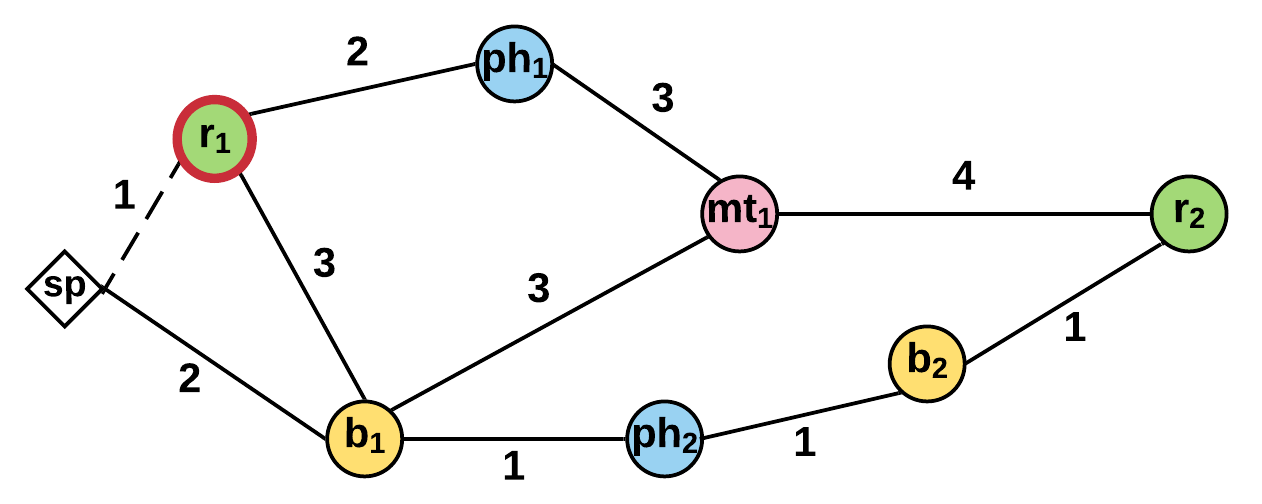
\includegraphics[scale=0.8]{Example_NEO_1.png}
	\end{figure}
	
	\begin{table}[h]
		\centering
		\begin{tabular}{ |l|p{10cm}| } 
			\hline
			Step & Heap contents (PSR $R : length(R)$) \\
			\hline
			\textcolor{red}{1} & \textcolor{red}{$(r_1 : 1)$} \\ 
			\hline
		\end{tabular}
	\end{table}

\end{frame}

\begin{frame}[noframenumbering]{Example: Step 2}
	$M = (r, ph, r)$, $UNEQUAL(0, 2)$
	
	\begin{figure}[h]
		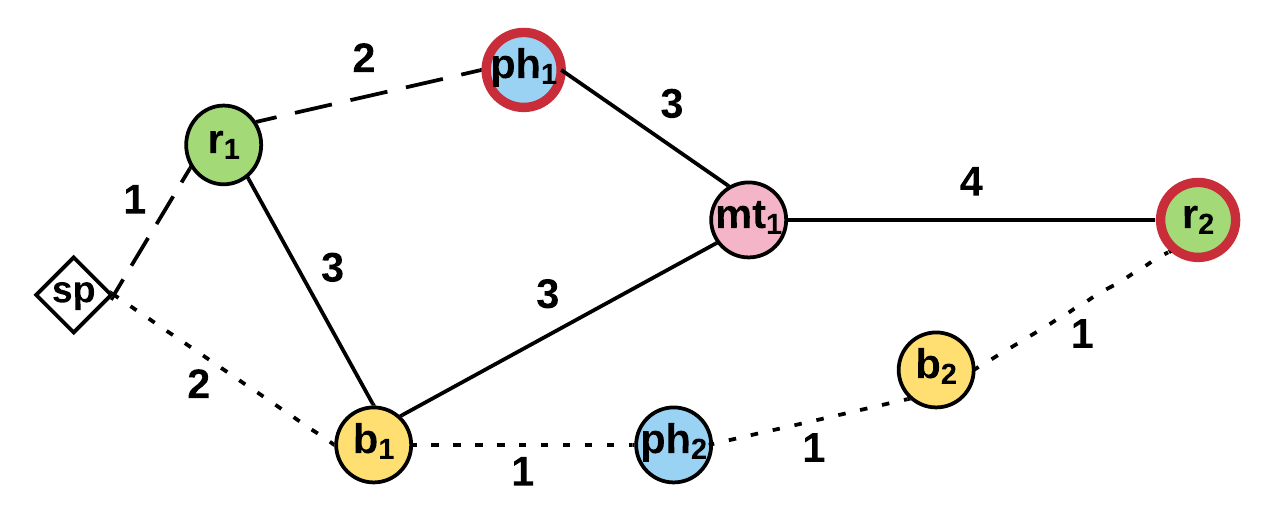
\includegraphics[scale=0.8]{Example_NEO_2.png}
	\end{figure}
	
	\begin{table}[h]
		\centering
		\begin{tabular}{ |l|p{10cm}| } 
			\hline
			Step & Heap contents (PSR $R : length(R)$) \\
			\hline
			1 & $(r_1 : 1)$ \\ 
			\hline
			\textcolor{red}{2} & \textcolor{red}{$(r_1, ph_1 : 3)$}, \textcolor{red}{$(r_2 : 5)$} \\ 
			\hline
		\end{tabular}
	\end{table}

\end{frame}

\begin{frame}[noframenumbering]{Example: Step 3}
	$M = (r, ph, r)$, $UNEQUAL(0, 2)$
	
	\begin{figure}[h]
		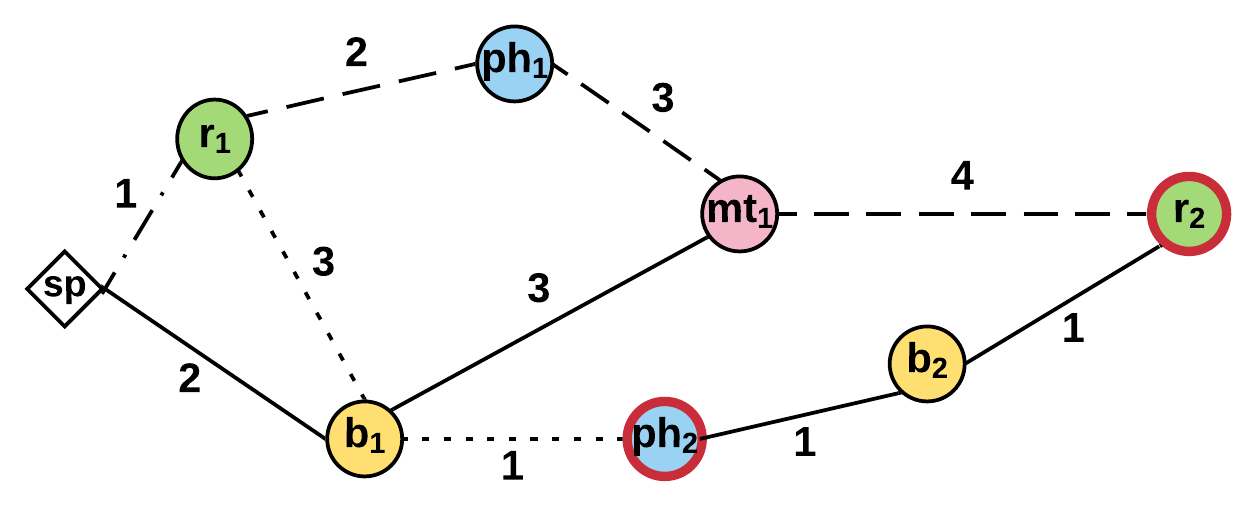
\includegraphics[scale=0.8]{Example_NEO_3.png}
	\end{figure}
	
	\begin{table}[h]
		\centering
		\begin{tabular}{ |l|p{10cm}| } 
			\hline
			Step & Heap contents (PSR $R : length(R)$) \\
			\hline
			2 & $(r_1, ph_1 : 3), (r_2 : 5)$ \\ 
			\hline
			\textcolor{red}{3} & $(r_2 : 5), $ \textcolor{red}{$(r_1, ph_2 : 5)$}, \textcolor{red}{$(r_1, ph_1, r_2 : 10)$} \\
			\hline 
		\end{tabular}
	\end{table}

\end{frame}

\begin{frame}[noframenumbering]{Example: Step 5}
	$M = (r, ph, r)$, $UNEQUAL(0, 2)$
	
	\begin{figure}[h]
		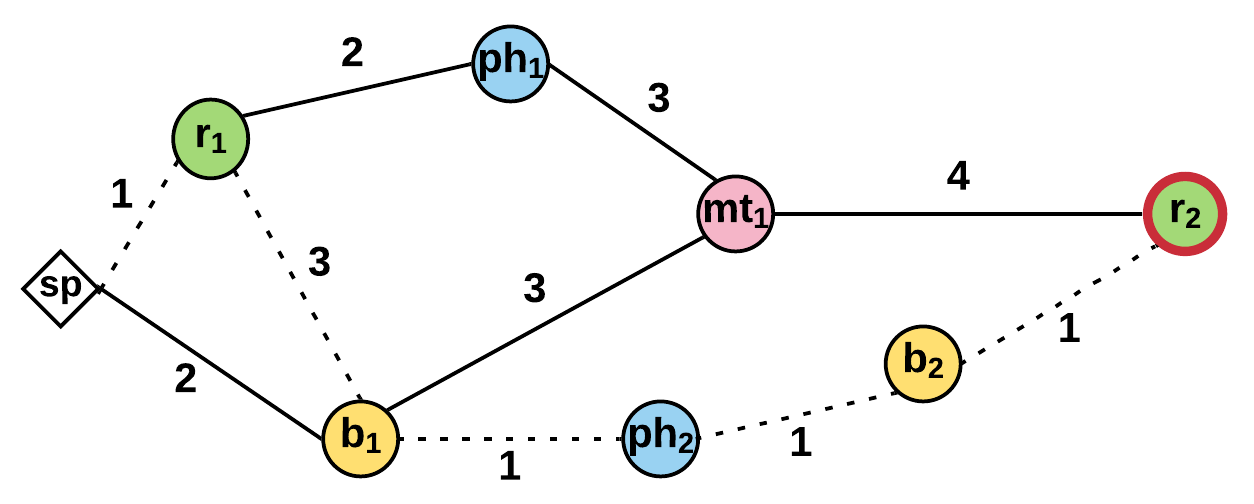
\includegraphics[scale=0.8]{Example_NEO_5.png}
	\end{figure}
	
	\begin{table}[h]
		\centering
		\begin{tabular}{ |l|p{10cm}| } 
			\hline
			Step & Heap contents (PSR $R : length(R)$) \\
			\hline
			4 & $(r_1, ph_2 : 5), (r_2, ph_2 : 7), (r_1, ph_1, r_2 : 10)$ \\ 
			\hline
			\textcolor{red}{5} & \textcolor{red}{$(r_1, ph_2, r_2 : 7)$}, $(r_2, ph_2 : 7),$ \st{$(r_1, ph_1, r_2 : 10)$} \\ 
			\hline
		\end{tabular}
	\end{table}

\end{frame}

%\begin{frame}{Example}
%	\begin{table}[]
%		\centering
%		\begin{tabular}{ |l|l| } 
%			\hline
%			Step & Heap contents (PSR $R : length(R)$) \\
%			\hline
%			1 & $(r_1 : 1)$ \\ 
%			\hline
%			2 & $(r_1, ph_1 : 3), (r_2 : 5)$ \\ 
%			\hline
%			3 & $(r_2 : 5), (r_1, ph_2 : 5), (r_1, ph_1, r_2 : 10)$ \\ 
%			\hline
%			4 & $(r_1, ph_2 : 5), (r_2, ph_2 : 7), (r_1, ph_1, r_2 : 10)$ \\ 
%			\hline
%			5 & $(r_1, ph_2, r_2 : 7), (r_2, ph_2 : 7), (r_1, ph_1, r_2 : 10)$ \\ 
%			\hline
%		\end{tabular}
%	\end{table}
%\end{frame}
	
	\subsection{Or operator}
		\begin{frame}{"Or" operator}
		
			\begin{itemize}
				\item \textbf{OR sequence:} An OR sequence $OR = (M_1, M_2, ..., M_m)$ represents the disjunction of category sequences, such as $M_1 = (c_1, c_2, ..., c_l)$.\newline
				\item \textit{Input}: A sequence of OR sequences $S = (OR_1, OR_2, ..., OR_n)$ and a starting point $sp$ in ${\rm I\!R}^2$
				\item \textit{Output}: Optimal route $R = (r_1, r_2, ..., r_l)$ \newline
				\pause
				\item \textbf{Proposed approach}: progressively inspects each option $M_i$ from the OR sequences $OR_i$ in \newline $S = (OR_1, OR_2, ..., OR_n)$, compares them and continues with the best one, based on length, until it reaches a full sequenced route
				\item \textbf{Proposed approach}: runs the PNE algorithm on all possible combinations of the query to find the shortest route out of them
			\end{itemize}
		
		\end{frame}
	
		%\begin{frame}{Example: Step 1}
	$S = (OR_1, OR_2, OR_3)$, $OR_1 = ((b), (ph))$, $OR_2 = ((mt))$, $OR_2 = ((r))$
	
	\begin{figure}[h]
		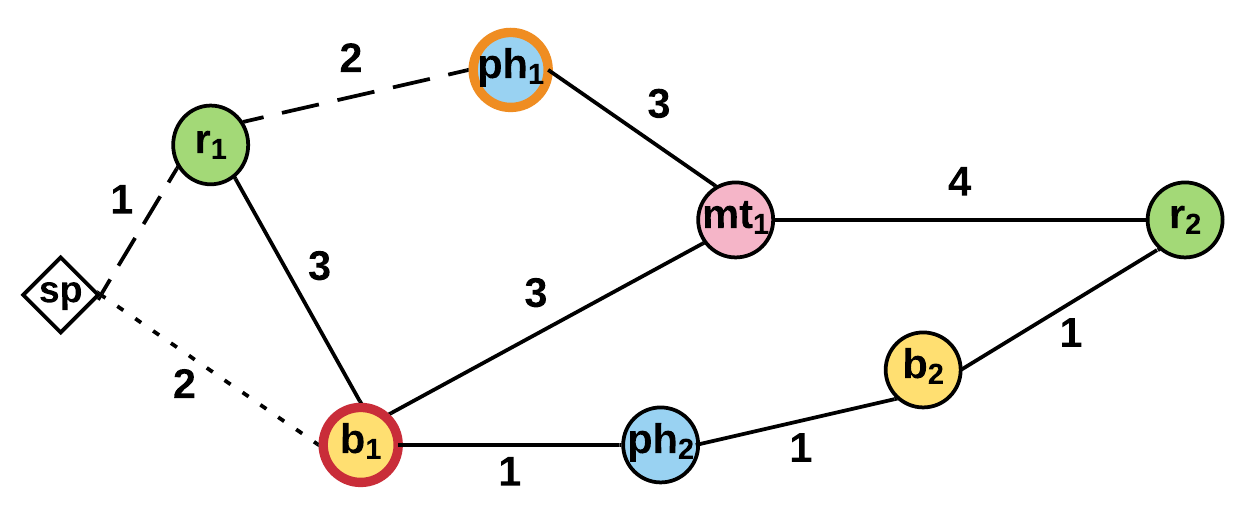
\includegraphics[scale=0.8]{Example_OR_1.png}
	\end{figure}
	
	\begin{table}[h]
		\centering
		\begin{tabular}{ |l|p{10cm}| } 
			\hline
			Step & Heap contents (PSR $R : length(r), index(R)$) \\
			\hline
			\textcolor{red}{1} & \textcolor{red}{$(b_1 : 2, 1)$} \\ 
			\hline
		\end{tabular}
	\end{table}

\end{frame}

\begin{frame}{Example: Step 2}
	$S = (OR_1, OR_2, OR_3)$, $OR_1 = ((b), (ph))$, $OR_2 = ((mt))$, $OR_2 = ((r))$
	
	\begin{figure}[h]
		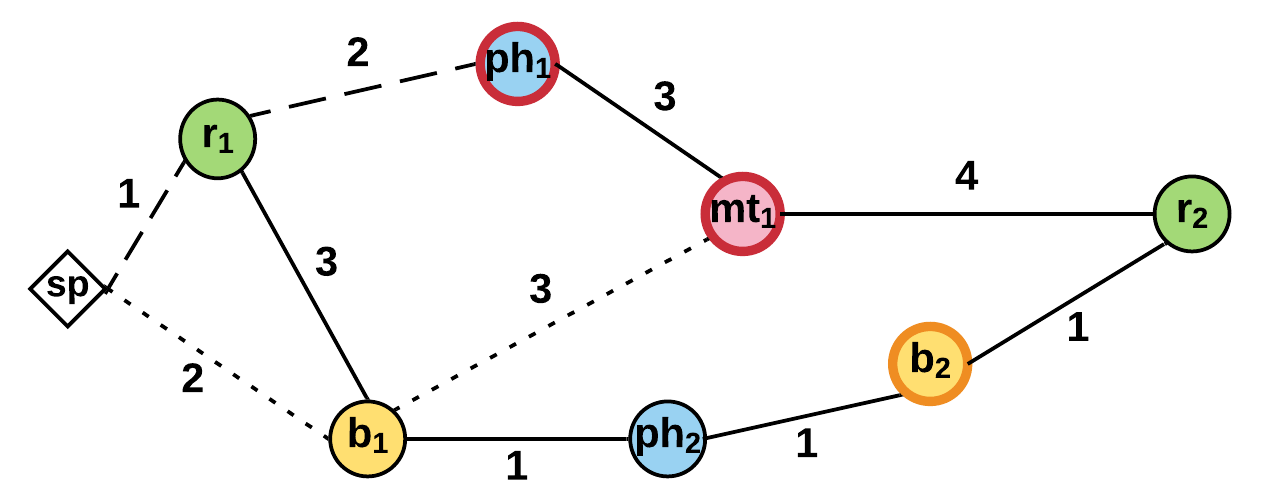
\includegraphics[scale=0.8]{Example_OR_2.png}
	\end{figure}
	
	\begin{table}[h]
		\centering
		\begin{tabular}{ |l|p{10cm}| } 
			\hline
			Step & Heap contents (PSR $R : length(r), index(R)$) \\
			\hline
			1 & $(b_1 : 2, 1)$ \\ 
			\hline
			\textcolor{red}{2} & \textcolor{red}{$(ph_1 : 3, 1)$}, \textcolor{red}{$(b_1, mt_1 : 5, 2)$} \\ 
			\hline
		\end{tabular}
	\end{table}

\end{frame}

\begin{frame}{Example: Step 6}
	$S = (OR_1, OR_2, OR_3)$, $OR_1 = ((b), (ph))$, $OR_2 = ((mt))$, $OR_2 = ((r))$
	
	\begin{figure}[h]
		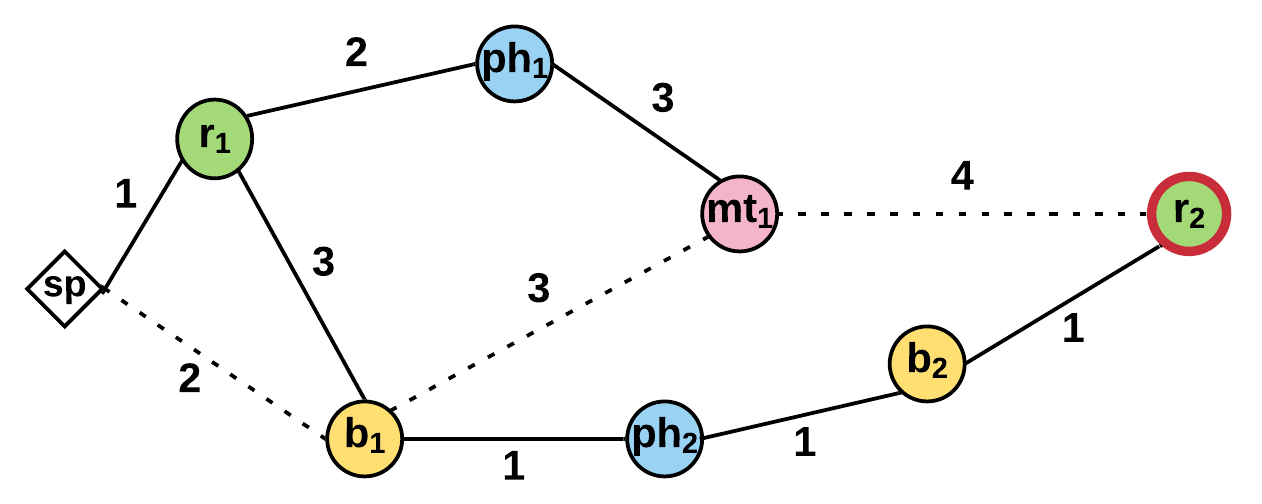
\includegraphics[scale=0.8]{Example_OR_6.png}
	\end{figure}
	
	\begin{table}[h]
		\centering
		\begin{tabular}{ |l|p{10cm}| } 
			\hline
			Step & Heap contents (PSR $R : length(r), index(R)$) \\
			\hline
			5 & $(b_1, mt_1 : 5, 2), (ph_1, mt_1 : 6, 2), (ph_2, mt_1 : 7, 2), (b_2, mt_1 : 9, 2)$ \\ 
			\hline
			\textcolor{red}{6} & $(ph_1, mt_1 : 6, 2), (ph_2, mt_1 : 7, 2), \textcolor{red}{(b_1, mt_1, r_2 : 9, 3)}, (b_2, mt_1 : 9, 2)$ \\ 
			\hline
		\end{tabular}
	\end{table}

\end{frame}

\begin{frame}{Example: Step 7}
	$S = (OR_1, OR_2, OR_3)$, $OR_1 = ((b), (ph))$, $OR_2 = ((mt))$, $OR_2 = ((r))$
	
	\begin{figure}[H]
		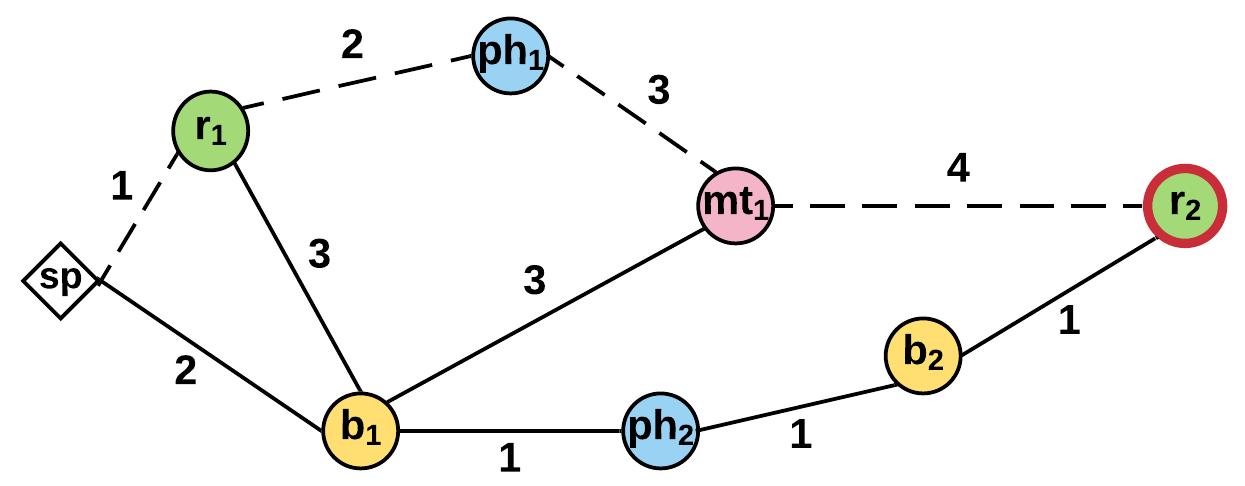
\includegraphics[scale=0.8]{Example_OR_7.png}
	\end{figure}
	
	\begin{table}[H]
		\centering
		\begin{tabular}{ |l|p{10cm}| } 
			\hline
			Step & Heap contents (PSR $R : length(r), index(R)$) \\
			\hline
			6 & $(ph_1, mt_1 : 6, 2), (ph_2, mt_1 : 7, 2), (b_1, mt_1, r_2 : 9, 3), (b_2, mt_1 : 9, 2)$ \\ 
			\hline
			\textcolor{red}{7} & $(ph_2, mt_1 : 7, 2), (b_1, mt_1, r_2 : 9, 3), (b_2, mt_1 : 9, 2),$ \textcolor{red}{\st{$(ph_1, mt_1, r_2 : 10, 3)$}} \\ 
			\hline
			8 & $(b_1, mt_1, r_2 : 9, 3), (b_2, mt_1 : 9, 2),$ \st{$(ph_2, mt_1, r_2 : 11, 3)$} \\ 
			\hline
		\end{tabular}
	\end{table}

\end{frame}

%\begin{frame}{Example}
%	\begin{table}[]
%		\centering
%		\begin{tabular}{ |l|p{10cm}| } 
%			\hline
%			Step & Heap contents (PSR $R : length(r), index(R)$) \\
%			\hline
%			1 & $(b_1 : 2, 1)$ \\ 
%			\hline
%			2 & $(ph_1 : 3, 1), (b_1, mt_1 : 5, 2)$ \\ 
%			\hline
%			3 & $(ph_2 : 3, 1), (ph_1, mt_1 : 6, 2), (b_1, mt_1 : 5, 2)$ \\ 
%			\hline
%			4 & $(b_2 : 4, 1), (b_1, mt_1 : 5, 2), (ph_1, mt_1 : 6, 2), (ph_2, mt_1 : 7, 2)$ \\ 
%			\hline
%			5 & $(b_1, mt_1 : 5, 2), (ph_1, mt_1 : 6, 2), (ph_2, mt_1 : 7, 2), (b_2, mt_1 : 9, 2)$ \\ 
%			\hline
%			6 & $(ph_1, mt_1 : 6, 2), (ph_2, mt_1 : 7, 2), (b_1, mt_1, r_2 : 9, 3), (b_2, mt_1 : 9, 2)$ \\ 
%			\hline
%			7 & $(ph_2, mt_1 : 7, 2), (b_1, mt_1, r_2 : 9, 3), (b_2, mt_1 : 9, 2),$ \st{$(ph_1, mt_1, r_2 : 10, 3)$} \\ 
%			\hline
%			8 & $(b_1, mt_1, r_2 : 9, 3), (b_2, mt_1 : 9, 2),$ \st{$(ph_2, mt_1, r_2 : 11, 3)$} \\ 
%			\hline
%		\end{tabular}
%	\end{table}
%\end{frame}
	
	\subsection{Order operator}
		\begin{frame}{"Order" operator}
		
			\begin{itemize}
				\item \textbf{ORDER sequence:} An order sequence $ORDER = (i_1, i_2, ..., i_k)$, is a sequence of indices in a category sequence $M = (c_1, c_2, ..., c_l)$, which indicate that the categories at the given indices should remain in the fixed positions in this category sequence.
				%\item $NOTORDERED = \overline{ORDER}$ 
				\item \textit{Input}: A sequence of categories $M = (c_1, c_2, ..., c_l)$, a starting point $sp$ in ${\rm I\!R}^2$ and an ORDER sequence $ORDER = (i_1, i_2, ..., i_k)$
				\item \textit{Output}: Optimal route $R = (r_1, r_2, ..., r_l)$ \newline
				\pause
				\item \textbf{Proposed approach}: inspects progressively each category option for the indices out of the NOTORDERED sequence, compares them and continues with the best one, based on length, until it reaches a full sequenced route.
				\item \textbf{Proposed approach}: runs the PNE algorithm on all possible permutations of the query to find the shortest route out of them
			\end{itemize}
		
		\end{frame}
	
		%\begin{frame}{Example: Step 1}
	$M = (b, r, ph)$, $ORDER = (1)$
	
	\begin{figure}[h]
		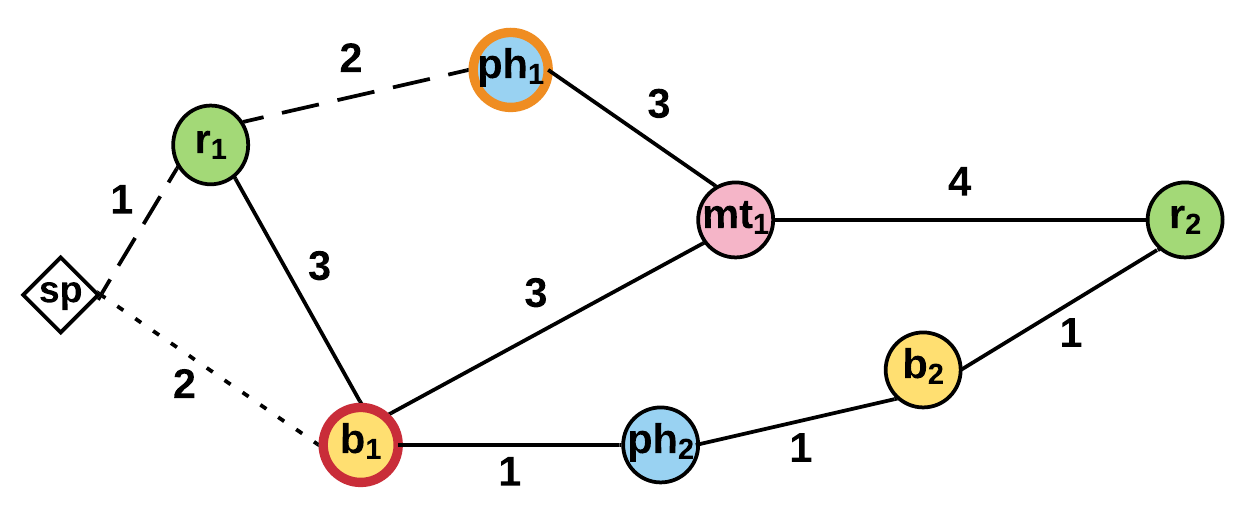
\includegraphics[scale=0.8]{Example_OR_1.png}
	\end{figure}
	
	\begin{table}[h]
		\centering
		\begin{tabular}{ |l|p{10cm}| } 
			\hline
			Step & Heap contents (PSR $R : length(r), r.notordered$) \\
			\hline
			\textcolor{red}{1} & \textcolor{red}{$(b_1 : 2, [ph])$} \\ 
			\hline
		\end{tabular}
	\end{table}

\end{frame}

\begin{frame}{Example: Step 1}
	$M = (b, r, ph)$, $ORDER = (1)$
	
	\begin{figure}[h]
		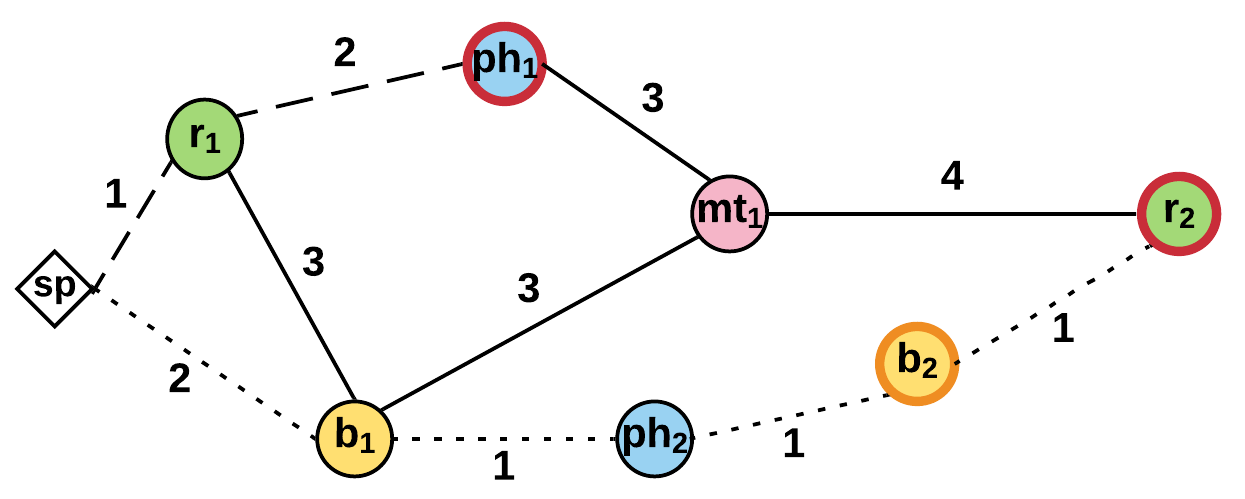
\includegraphics[scale=0.8]{Example_ORDER_2.png}
	\end{figure}
	
	\begin{table}[h]
		\centering
		\begin{tabular}{ |l|p{10cm}| } 
			\hline
			Step & Heap contents (PSR $R : length(r), r.notordered$) \\
			\hline
			1 & $(b_1 : 2, [ph])$ \\ 
			\hline
			\textcolor{red}{2} & \textcolor{red}{$(ph_1 : 3, [b])$}, \textcolor{red}{$(b_1, r_2 : 5, [ph])$} \\ 
			\hline
		\end{tabular}
	\end{table}

\end{frame}

\begin{frame}{Example: Step 6}
	$M = (b, r, ph)$, $ORDER = (1)$
	
	\begin{figure}[h]
		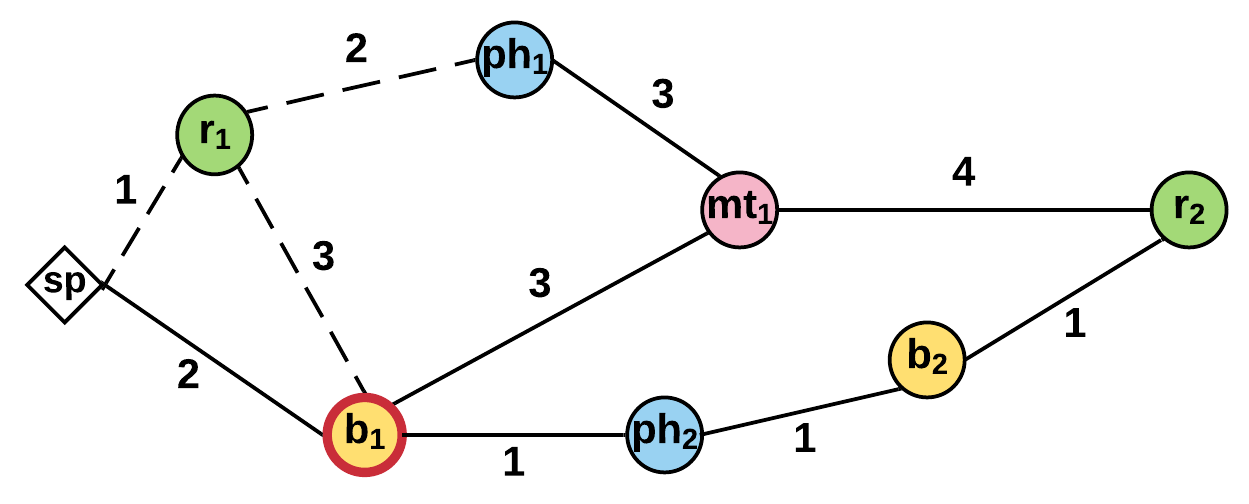
\includegraphics[scale=0.8]{Example_ORDER_6.png}
	\end{figure}
	
	\begin{table}[h]
		\centering
		\begin{tabular}{ |l|p{10cm}| } 
			\hline
			Step & Heap contents (PSR $R : length(r), r.notordered$) \\
			\hline
			5 & $(ph_1, r_1 : 5, [b]), (b_2, r_2 : 5, [ph]), (ph_2, r_2 : 5, [b]), (b_1, r_2 : 5, [ph])$ \\ 
			\hline
			\textcolor{red}{6} & $(b_2, r_2 : 5, [ph]), (ph_2, r_2 : 5, [b]), (b_1, r_2 : 5, [ph]),$ \textcolor{red}{$(ph_1, r_1, b_1 : 8, [])$} \\ 
			\hline
		\end{tabular}
	\end{table}

\end{frame}

\begin{frame}{Example: Step 12}
	$M = (b, r, ph)$, $ORDER = (1)$
	
	\begin{figure}[h]
		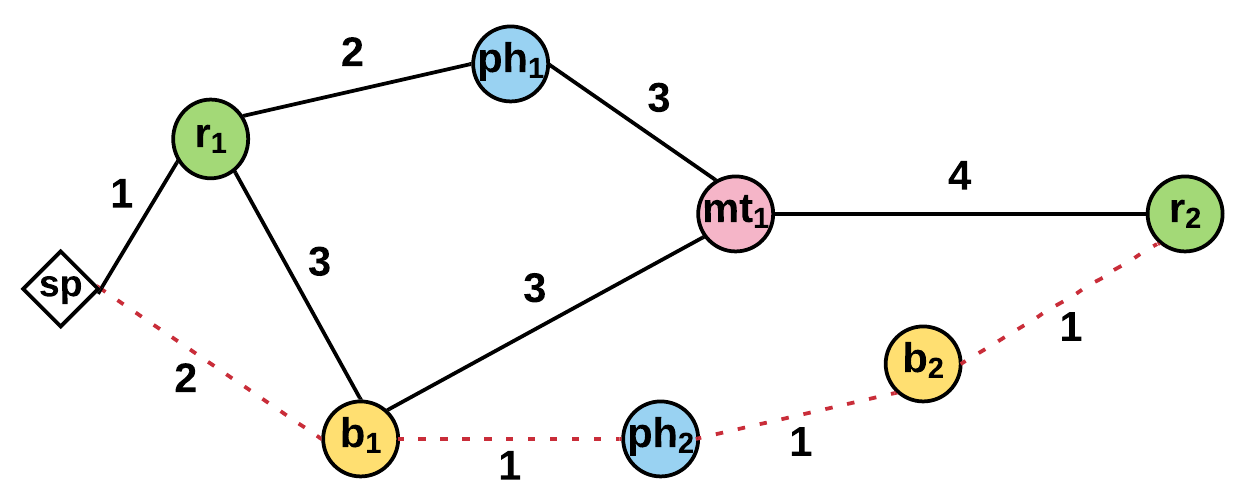
\includegraphics[scale=0.8]{Example_ORDER_12.png}
	\end{figure}
	
	\begin{table}[h]
		\centering
		\begin{tabular}{ |l|p{10cm}| } 
			\hline
			Step & Heap contents (PSR $R : length(r), r.notordered$) \\
			\hline
			10 & $(b_2, r_2 : 5, [ph]), (ph_2, r_2, b_2 : 6, []),$ \st{$(b_1, r_1, ph_1 : 7, [])$} $, (ph_2, r_1 :7, [b]), (b_2, r_1 : 9, [ph]), (ph_1, r_2 : 10, [b])$ \\ 
			\hline
			11 & $\textcolor{red}{(ph_2, r_2, b_2 : 6, [])}, (ph_2, r_1 :7, [b]), (b_2, r_1 : 9, [ph]), (ph_1, r_2 : 10, [b]),$ \st{$(b_2, r_2, ph_1 : 12, [])$} \\ 
			\hline
		\end{tabular}
	\end{table}

\end{frame}

\begin{frame}{Example}
	\begin{table}[]
		\centering
		\begin{tabular}{ |l|p{10cm}| } 
			\hline
			Step & Heap contents (PSR $R : length(r), r.notordered$) \\
			\hline
			1 & $(b_1 : 2, [ph])$ \\ 
			\hline
			2 & $(ph_1 : 3, [b]), (b_1, r_2 : 5, [ph])$ \\ 
			\hline
			3 & $(ph_2 : 3, [b]), (ph_1, r_1 : 5, [b]), (b_1, r_2 : 5, [ph])$ \\ 
			\hline
			4 & $(b_2 : 4, [ph]), (ph_2, r_2 : 5, [b]), (ph_1, r_1 : 5, [b]), (b_1, r_2 : 5, [ph])$ \\ 
			\hline
			5 & $(ph_1, r_1 : 5, [b]), (b_2, r_2 : 5, [ph]), (ph_2, r_2 : 5, [b]), (b_1, r_2 : 5, [ph])$ \\ 
			\hline
			6 & $(b_2, r_2 : 5, [ph]), (ph_2, r_2 : 5, [b]), (b_1, r_2 : 5, [ph]), (ph_1, r_1, b_1 : 8, [])$ \\ 
			\hline
			7 & $(b_1, r_2 : 5, [ph]), (b_2, r_2, ph : 5, [ph]), (ph_2, r_2 : 5, [b]), (b_2, r_2, ph_2 : 7, []),$ \st{$(ph_1, r_1, b_1 : 8, [])$} $, (b_2, r_1 : 9, [ph]), (ph_1, r_2 : 10, [b])$ \\ 
			\hline
			8 & $(b_2, r_2 : 5, [ph]), (ph_2, r_2 : 5, [b]), (b_1, r_1 : 5, [ph]), (b_2, r_2, ph_2 : 7, []), $ \st{$(b_1, r_2, ph_2 : 7, [])$} $, (b_2, r_1 : 9, [ph]), (ph_1, r_2 : 10, [b])$ \\ 
			\hline
			9 & $(b_1, r_1 : 5, [ph]), (b_2, r_2 : 5, [ph]), (ph_2, r_2, b_2 : 6, []),$ \st{$(b_2, r_2, ph_2 : 7, [])$} $, (ph_2, r_1 :7, [b]), (b_2, r_1 : 9, [ph]), (ph_1, r_2 : 10, [b])$ \\ 
			\hline
			10 & $(b_2, r_2 : 5, [ph]), (ph_2, r_2, b_2 : 6, []),$ \st{$(b_1, r_1, ph_1 : 7, [])$} $, (ph_2, r_1 :7, [b]), (b_2, r_1 : 9, [ph]), (ph_1, r_2 : 10, [b])$ \\ 
			\hline
			11 & $(ph_2, r_2, b_2 : 6, []), (ph_2, r_1 :7, [b]), (b_2, r_1 : 9, [ph]), (ph_1, r_2 : 10, [b]),$ \st{$(b_2, r_2, ph_1 : 12, [])$} \\ 
			\hline
		\end{tabular}
	\end{table}
\end{frame}
	
\section{Evaluation}

	\subsection{Experiments}
		\begin{frame}{Experiments}
		
			\begin{itemize}
				\item Road network of Berlin, with 428769
				crossroad nodes, 504229 road edges, 5548 PoIs and 7 category types
				\item 1000 queries with randomly selected
				starting points
			\end{itemize}
		
			\begin{table}[H]
				\centering
				\begin{tabular}{ |c|c|c| } 
					\hline
					\textit{Categories} & \textit{Size} & \textit{Frequency}\\
					\hline
					Restaurants & 2081 & \multirow{3}{3em}{High}\\ 
					Coffee shops & 1002 &\\
					Pubs and bars & 958 &\\  
					\hline
					Atms/Banks & 597 & \multirow{3}{3em}{Middle}\\
					Pharmacies & 589 &\\
					\hline
					Gas stations & 180 & \multirow{3}{3em}{Low}\\
					Movie theaters & 141 &\\ 
					\hline
				\end{tabular}
				
			\end{table}
	
			\begin{itemize}
				\item \textbf{Quantitative evaluation criteria}: run time, number of heap fetches, maximum heap size (work space)
				\item \textbf{Qualitative evaluation}: compare against baseline approaches
			\end{itemize}
		
		\end{frame}

	\subsection{Equality operator}
		\begin{frame}{"Equality" operator - query length}
		
			\begin{itemize}
				\item \textbf{Evaluation parameters}: (1) query length, (2) frequency of the categories $c_i$, $c_j$ in the category sequence and (3) distance between the categories $c_i$, $c_j$
			\end{itemize}
		
			\begin{figure}[h]
				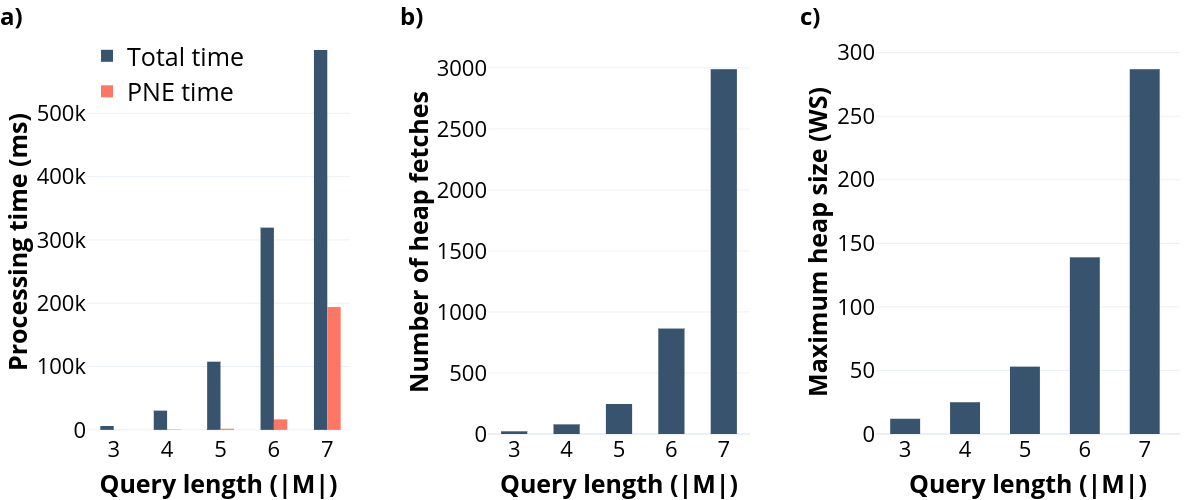
\includegraphics[scale=0.275]{eo_length_orange.png}
			\end{figure}
		
		\end{frame}
	
		\begin{frame}{"Equality" operator - category frequency}
		
			\begin{itemize}
				\item \textbf{Evaluation parameters}: (1) query length, (2) frequency of the categories $c_i$, $c_j$ in the category sequence and (3) distance between the categories $c_i$, $c_j$
			\end{itemize}
			
			\begin{figure}[h]
				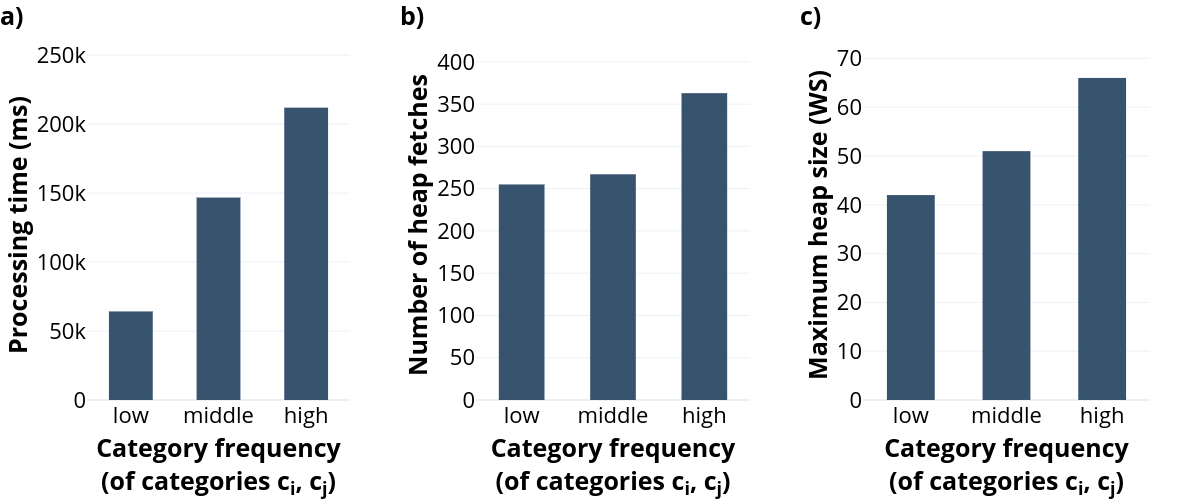
\includegraphics[scale=0.275]{eo_frequency.png}
			\end{figure}
		
		\end{frame}
	
		\begin{frame}{"Equality" operator - category distance}
		
			\begin{itemize}
				\item \textbf{Evaluation parameters}: (1) query length, (2) frequency of the categories $c_i$, $c_j$ in the category sequence and (3) distance between the categories $c_i$, $c_j$
			\end{itemize}
			
			\begin{figure}[h]
				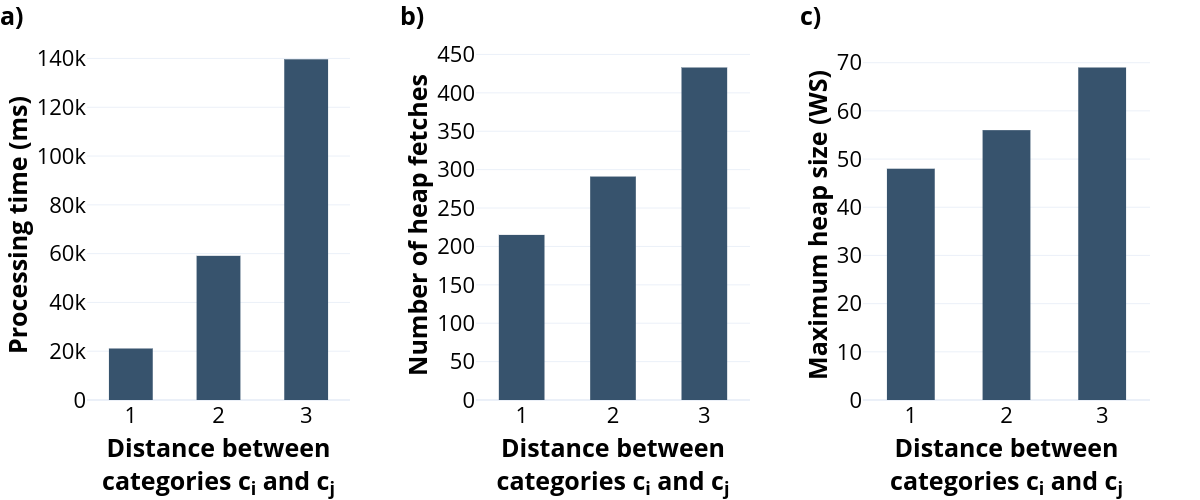
\includegraphics[scale=0.275]{eo_distance.png}
			\end{figure}
		
		\end{frame}
	
		\begin{frame}{"Equality" operator - baseline approach}
			
			\begin{figure}[h]
				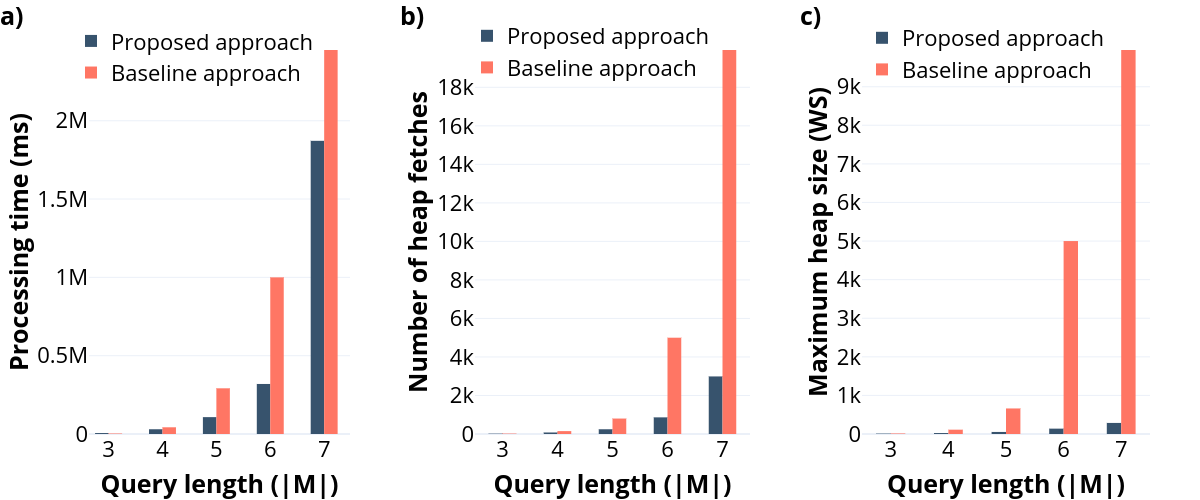
\includegraphics[scale=0.275]{eo2.png}
			\end{figure}
		
		\end{frame}
		
	\subsection{Inequality operator}
		\begin{frame}{"Inequality" operator - query length}
		
			\begin{itemize}
				\item \textbf{Evaluation parameters}: (1) query length, (2) frequency of the categories $c_i$, $c_j$ in the category sequence and (3) distance between the categories $c_i$, $c_j$
			\end{itemize}
		
			\begin{figure}[h]
				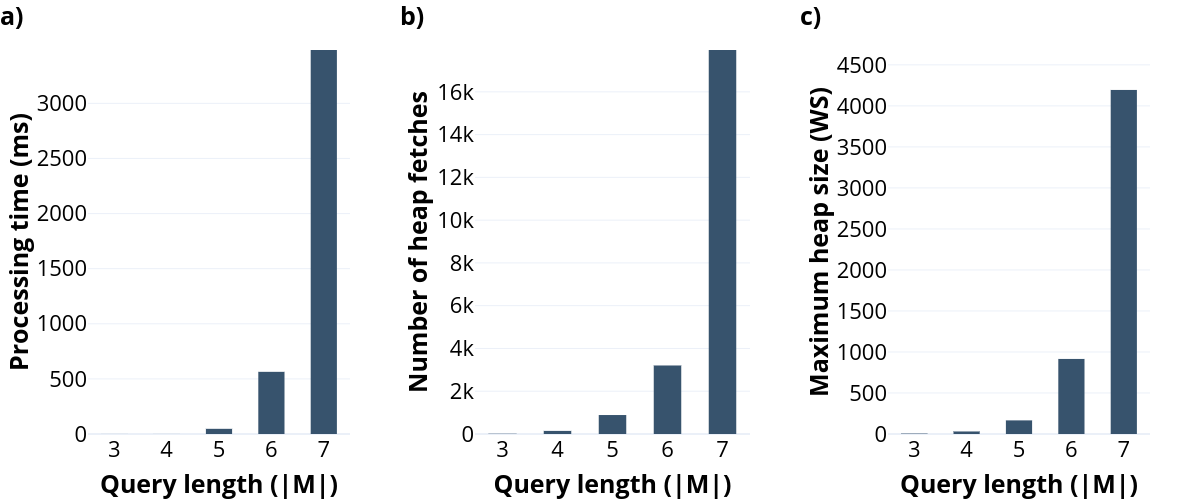
\includegraphics[scale=0.275]{neo_length.png}
			\end{figure}
		
		\end{frame}
	
	\subsection{Or operator}
		\begin{frame}{"Or" operator}
		
			\begin{itemize}
				\item \textbf{Evaluation parameter}: type and number of operands
				\begin{itemize}
					\item simple OR operand: $|M| = 1$
					\item complex OR operand: $|M| > 1$
				\end{itemize}
			\end{itemize}
		
			\begin{figure}[H]
				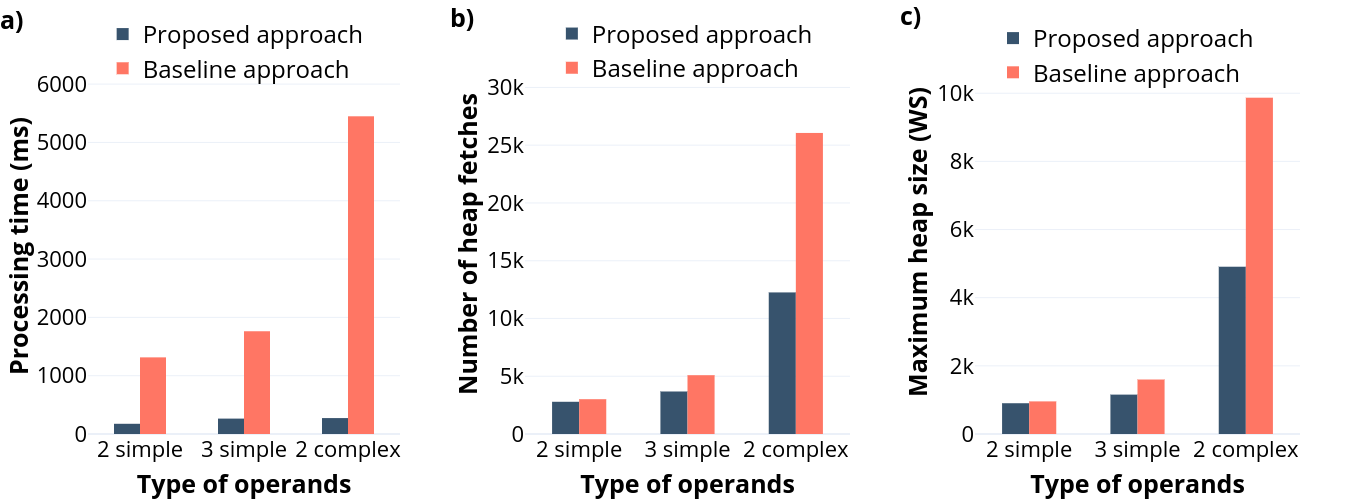
\includegraphics[scale=0.25]{or.png}
			\end{figure}
		
		\end{frame}
	
	\subsection{Order operator}
		\begin{frame}{"Order" operator}
		
			\begin{itemize}
				\item \textbf{Evaluation parameter}: number of fixed positions in $M$
			\end{itemize}
			
			\begin{figure}[h]
				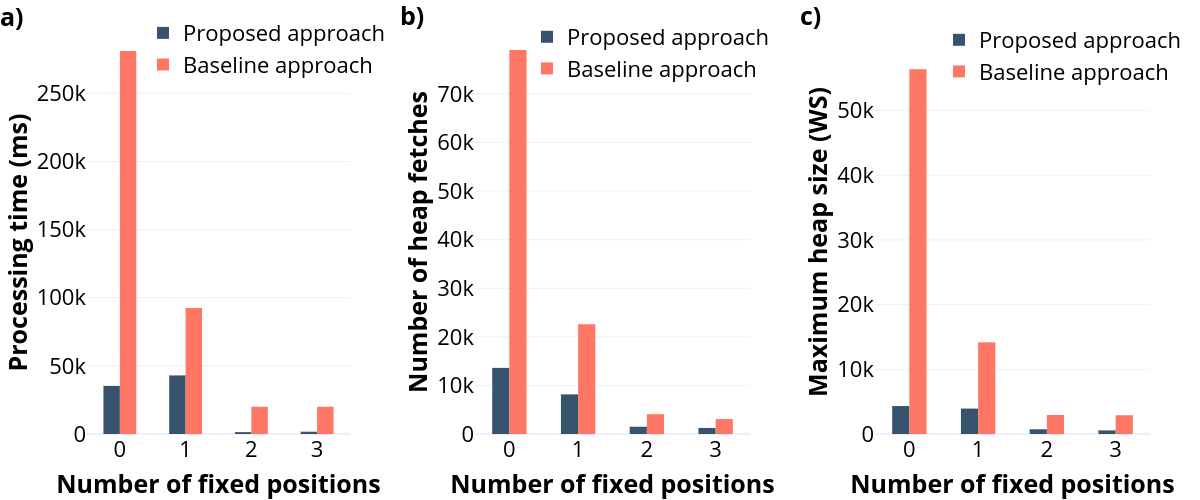
\includegraphics[scale=0.275]{order.png}
			\end{figure}
		
		\end{frame}
	
\section{Conclusion}
	\begin{frame}{Conclusion}
	
		\begin{itemize}
			\item Proposed four essential route query language operators 
			\item Developed algorithms that deliver an optimal result in metric spaces
			\item Evaluated the approaches qualitatively and quantitatively and proved the efficiency of the algorithms
			\
		\end{itemize}
	
	\end{frame}

\section{Discussion}
	\begin{frame}{Discussion and Future Work}
	
		\begin{itemize}
			\item Easily modified: using a different quantifying parameter such as travel duration, finding $k$ optimal routes
			\item Additional operators are possible: "hop", "and", "not", "necessity"
			\item A different approach to implementing the operators
				\begin{itemize}
					\item Skyline concept \cite{skyline}
				\end{itemize}
			\item Extending the proposed algorithms to also support dynamic road networks, in which traffic information is provided (e.g., travel time, traffic congestion, etc.). \cite{dynamic}
		\end{itemize}
	
	\end{frame}

	\begin{frame}{The End}
		\centering \Large
		\emph{\textcolor{kit}{Thank you for the attention!}}
	\end{frame}


%			\begin{block}{Aktivieren}
%				\begin{itemize}
%					\item "Hey, Siri"
%					\item Home-Knopf
%				\end{itemize}
%			\end{block}
%		
%			\begin{exampleblock}{Unterstützte Funktionen}
%				\begin{itemize}
%					\item Handyspezifische Funktionen wie Anrufe, Erinnerungen und Kalendereinträge
%					\item Anfragen, die Webservices voraussetzen, wie Wettervorhersage, Route finden und triviale Suchmaschinenfragen
%				\end{itemize}
%			\end{exampleblock}
%		
%			\begin{alertblock}{Zusätzliche Funktionen}
%				\begin{itemize}
%					\item Mittels der VoiceOver Funktion wird der Bildschirminhalt laut gelesen
%					\item Lustige Antworten auf philosophische und kontroverse Fragen
%				\end{itemize}
%			\end{alertblock}
%		

\appendix

\begin{frame}[allowframebreaks]{Literatur}

	%% --------------------
	%% |   Bibliography   |
	%% --------------------
	
	\bibliographystyle{alphadin}	% german style
	
	\section{Literatur}
	\begin{thebibliography}{9}
		
		\bibitem{tpq} 
		Feifei Li, Dihan Cheng, Marios Hadjieleftheriou, George Kollios and Shang-Hua Teng.
		\textit{On trip planning queries in spatial databases}. 
		In Bauzer Medeiros C., Egenhofer M.J., Bertino E. (eds) Advances in Spatial and Temporal Databases (SSTD), pages 273–290, 2005.
		
		\bibitem{osr} 
		Mehdi Sharifzadeh, Mohammad Kolahdouzan and Cyrus Shahabi.
		\textit{The optimal sequenced route query}. 
		The VLDB Journal, 17:765–787, 2008.
		
		\bibitem{skyline} 
		Yuya Sasaki, Yoshiharu Ishikawa, Yasuhiro Fujiwara and Makoto Onizuka.
		\textit{Sequenced route query with semantic hierarchy}. 
		In EDBT, pages 37–48, 2018.
		
		\bibitem{factors} 
		Jian Dai, Chengfei Liu, Jiajie Xu4 and Zhiming Ding.
		\textit{On personalized and sequenced route planning}. 
		World Wide Web, 19:679–705, 2016.
		
		\bibitem{moving} 
		Jochen Eisner and Stefan Funke.
		\textit{Sequenced route queries: Getting things done on the way back home}. 
		In SIGSPATIAL ’12 Proceedings of the 20th International Conference on Advances in Geographic Information Systems, pages 502–505, 2012.
		
		\bibitem{multi} 
		Haiquan Chen, Wei-Shinn Ku, Min-Te Sun and Roger Zimmermann.
		\textit{The partial sequenced route query with traveling rules in road networks}. 
		Geoinformatica, 15:541–569, 2011.
		
		\bibitem{dynamic} 
		Nirmesh Malviya, Samuel Madden and Arnab Bhattacharya. A continuous query system for dynamic route planning.
		\textit{A continuous query system for dynamic route planning}. 
		In ICDE ’11 Proceedings of the 2011 IEEE 27th International Conference on Data Engineering, pages 792–803, 2011.
		
	\end{thebibliography}
\end{frame}

\begin{frame}{Inequality operator - category frequency}

	\begin{itemize}
		\item \textbf{Evaluation parameters}: (1) query length, (2) frequency of the categories $c_i$, $c_j$ in the category sequence and (3) distance between the categories $c_i$, $c_j$
	\end{itemize}
	
	\begin{figure}[h]
		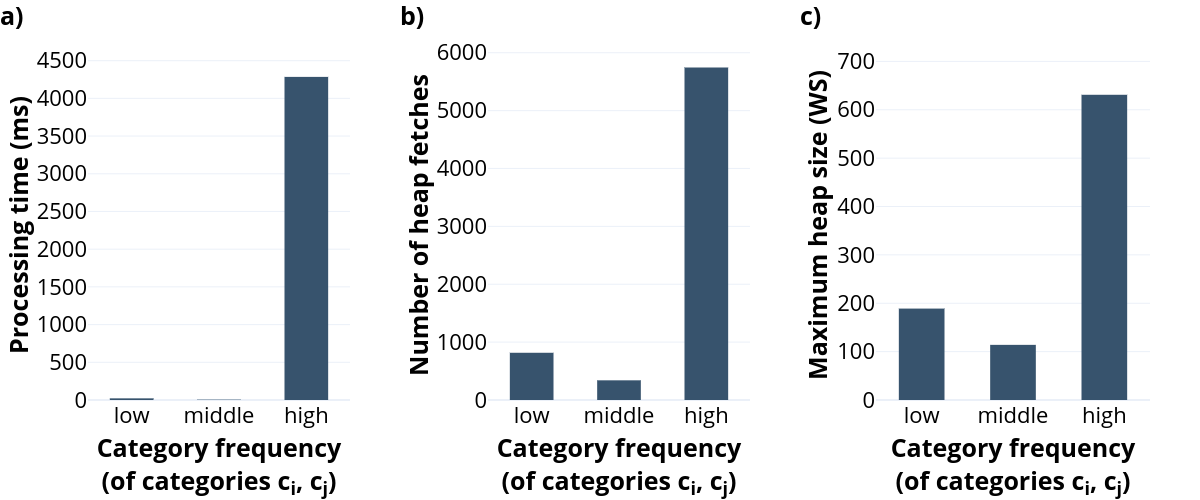
\includegraphics[scale=0.275]{neo_frequency.png}
	\end{figure}

\end{frame}

\begin{frame}{Inequality operator - category distance}

	\begin{itemize}
		\item \textbf{Evaluation parameters}: (1) query length, (2) frequency of the categories $c_i$, $c_j$ in the category sequence and (3) distance between the categories $c_i$, $c_j$
	\end{itemize}
	
	\begin{figure}[h]
		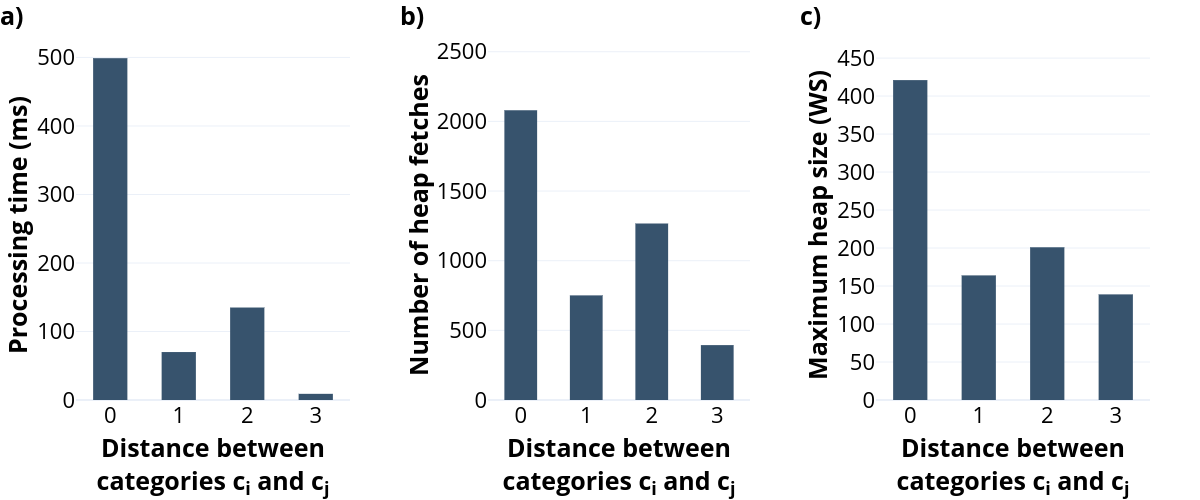
\includegraphics[scale=0.275]{neo_distance.png}
	\end{figure}

\end{frame}

\begin{frame}{PNE Algorithm}
\scalebox{.8}{\begin{algorithm}[H]
		\caption{PNE}
		fetch a $PSR$ from the heap\;
		\Switch{$s = size(PSR)$}{
			\Case{$s == l$}{
				$PSR$ is the optimal route\;
				\Return $PSR$\;
			}
			\Case{$s \neq l$}{
				\A{
					\NN{$r_{|PSR|}, C_{M_{|PSR|+1}}$}\;
					update $PSR$ and perform trimming in case it is a candidate SR \;
					put $PSR$ back on the $heap$ \;
				} 
				\B{
					\KNN{$r_{|PSR|-1}, C_{M_{|PSR|}}$}\;
					generate a new $PSR$ and place it on the $heap$\;
				} 
			}
		}
\end{algorithm}}
\end{frame}

\begin{frame}{Notations}

	\begin{table}[H]
		\centering
		\scalebox{.8}{\begin{tabular}{ |l|p{10cm}| } 
			\hline
			\textit{Symbol} & \textit{Meaning} \\
			\hline
			$C_i$ & a point set for a category in ${\rm I\!R}^2$ \\ 
			\hline
			$|C_i|$ & cardinality of the set $C_i$ \\ 
			\hline
			$n$ & number of point sets $C_i$ \\ 
			\hline
			$dist(., .)$ & distance function in ${\rm I\!R}^2$ \\ 
			\hline
			$M$ & category sequence, $=(c_1, c_2, ..., c_l)$ \\ 
			\hline
			$|M|$ & $l$, size of sequence $M$ = number of items in $M$ \\ 
			\hline
			$c_i$ & $i$th member of $M$ \\ 
			\hline
			$R$ & route, $= (r_1, r_2, ..., r_r)$ \\ 
			\hline
			$|R|$ & $r$, size of route $R$ = number of points in $R$ \\ 
			\hline
			$r_i$ & $i$th point in $R$ \\ 
			\hline
			$length(R)$ & length of $R$ \\ 
			\hline
			$length(sp, R)$ & length of $R_{sp} = (sp, r_1, r_2, ..., r_r)$, $= length(R_{sp})$ \\ 
			\hline
			$Q(sp, M)$ & sequenced route query \\ 
			\hline
			$NN(r_q, c_p)$ & nearest neighbor from the category point set $C_p$ to a route point $r_q$ \\ 
			\hline
			$KNN(r_q, c_p')$ & next nearest neighbor $r_p'$ from the category point set $C_p$ to a route point $r_q$ \\ 
			\hline
		\end{tabular}}
	\end{table}

\end{frame}

\begin{frame}{Modified PNE}

	\scalebox{.7}{\begin{algorithm}[H]
		\caption{modifiedPNE()}
		
		\ForEach(Checking the upper bound for every $r_1$ neighbor of $sp$ in the category set $C_{M_1}$){$r_1$ in $C_{M_1}$}{
			build a new $PSR$ with $r_1$\;
			\If{$LB(PSR) <= UB$}{
				place the new $PSR$ $(r_1)$ on the $heap$\;	
			}
		}
		
		\While{$heap$ is not empty}{
			$current \leftarrow$ fetch a $PSR$ from the $heap$\;
			\Switch{$s = size(current)$}{
				\Case(Finding PSRs before $r_j$){$s <= j-1$}{
					\caseBefore{}\;
				}
				\Case(Finding PSR containing $r_j$){$s = j$}{
					\caseContaining{}\;
				}
				\Case(Finding PSR after/containing $r_j$){$s = j+1$}{
					\caseAfterOrContaining{}\;
				}
				\Case(Finding PSRs after $r_j$){$s >= j+2$}{
					\caseAfter{}\;
				}
			}
		}
		
		\Return $foundSR$
		
	\end{algorithm}}

\end{frame}


\begin{frame}{NEO - Trimming}

	\scalebox{.7}{\begin{procedure}[H]
			\caption{trim($PSR$)}
			\label{proc:trim_NEO}
			
			\eIf{$size(PSR) = l$}{
				\eIf{$PSR[i] \neq PSR[j]$}{
					\tcp{Optimization: length check}
					\If{$length(PSR) <= length(candidate)$}{
						update $candidate$\;
						place $PSR$ on the $heap$\;
					}
				}
				{
					\tcp{In case $j$ is the last index in the route, we find the kth neighbor of the previous PoI to the last one}
					\If{$size(PSR) = j + 1$}{
						\KNN{$r_{|PSR|-1}, C_{M_{|PSR|}}$}\;
						generate a new $PSR$\;
						\trim{$PSR$}\;
					}
				}
				
			}{
				\tcp{Optimization: length check}
				\If{$length(PSR) <= length(candidate)$}{
					place $PSR$ on the $heap$\;
				}
			}
	\end{procedure}}

\end{frame}

\end{document}
